%%%%%%%%%%%%%%%%%%%%%%%%%%%%%%%%%%%%%%%%%%%%%%%%%%%%%%%%%%%%%
%% HEADER
%%%%%%%%%%%%%%%%%%%%%%%%%%%%%%%%%%%%%%%%%%%%%%%%%%%%%%%%%%%%%
\documentclass[a4paper,oneside,12pt]{report}

%% Language %%%%%%%%%%%%%%%%%%%%%%%%%%%%%%%%%%%%%%%%%%%%%%%%%
\usepackage[english]{babel}
%\usepackage[greek]{babel}
%\usepackage[utf8x]{inputenc}
\usepackage{lmodern} %Type1-font for non-english texts and characters
\usepackage[ansinew]{inputenc}
\usepackage[T1]{fontenc}
%\usepackage{kerkis}

%% Formatting %%%%%%%%%%%%%%%%%%%%%%%%%%%%%%%%%%%%%%%%%%%%%%%
\frenchspacing
\usepackage{parskip}
%\usepackage{fullpage}
\usepackage{a4wide}
%\usepackage{setspace}
\usepackage{titlesec} % Package to allow chapter number on the same line as chapter title
\titleformat{\chapter}[hang]  % Package to allow chapter number on the same line as chapter title
{\normalfont\huge\bfseries}{\chaptertitlename\ \thechapter:}{0.5em}{\filright} % Package to allow chapter number on the same line as chapter title

%\usepackage{subfig}

%% Packages for Graphics & Figures %%%%%%%%%%%%%%%%%%%%%%%%%%
\usepackage{graphicx}
\usepackage[section]{placeins}
\usepackage{float}
\restylefloat{table}
%%Float Adjustment
%two column float page must be 90% full
\renewcommand\dblfloatpagefraction{.90}
%two column top float can cover up to 80% of page
\renewcommand\dbltopfraction{.80}
%float page must be 90% full
\renewcommand\floatpagefraction{.90}
%top float can cover up to 80% of page
\renewcommand\topfraction{.80}
%bottom float can cover up to 80% of page
\renewcommand\bottomfraction{.80}
%at least X% of a normal page must contain text
\renewcommand\textfraction{.1}
%separation between floats and text
\setlength\dbltextfloatsep{9pt plus 5pt minus 3pt }
%separation between two column floats and text
\setlength\textfloatsep{4pt plus 2pt minus 1.5pt}
\usepackage{tikz}
\usetikzlibrary{arrows, shapes, automata,petri}

%% Math Packages %%%%%%%%%%%%%%%%%%%%%%%%%%%%%%%%%%%%%%%%%%%%
\usepackage{amsmath}
\usepackage{amsthm}
\usepackage{amsfonts}
\usepackage{bm}
\DeclareMathOperator{\Cov}{Cov}
\DeclareMathOperator{\Var}{Var}
\usepackage[retainorgcmds]{IEEEtrantools}

%% Packages for document interactivity
\usepackage{hyperref}
\hypersetup{
		colorlinks,
    citecolor=black,
    filecolor=black,
    linkcolor=black,
    urlcolor=black
}
\usepackage{url}
\usepackage[nottoc]{tocbibind} % Add the bibliography in the ToC

% Conditional content
\usepackage{versions} % Compile content conditionally
%\usepackage{etoolbox}

% Project automation
\usepackage[tocentry]{vhistory}

%% Other options to examine %%%%%%%%%%%%%%%%%%%%%%%%%%%%%%%%%
%\usepackage{usenames, dvipsnames]{color}
%\usepackage{amssymb}
%\usepackage{cclicenses}
%\usepackage{siunitx}
%\usepackage{ucs}
%\raggedbottom
\newcommand{\HRule}{\rule{\linewidth}{0.5mm}}
%\renewcommand{\labelenumi}{\roman{enumi}}
%\usepackage{sinunitx}


%%%%%%%%%%%%%%%%%%%%%%%%%%%%%%%%%%%%%%%%%%%%%%%%%%%%%%%%%%%%%
%% DOCUMENT
%%%%%%%%%%%%%%%%%%%%%%%%%%%%%%%%%%%%%%%%%%%%%%%%%%%%%%%%%%%%%
\begin{document}

\pagestyle{empty} %No headings for the first pages.


%% Title Page %%%%%%%%%%%%%%%%%%%%%%%%%%%%%%%%%%%%%%%%%%%%%%%
%%%%%%%%%%%%%% TITLE PAGE %%%%%%%%%%%%%%%%
%%%%%%%%%%%%%%%%%%%%%%%%%%%%%%%%%%%%%%%%%%
\begin{titlingpage}
\begin{center}


\includegraphics[width=0.3\textwidth]{./figures/ntua_logo}~\\[1cm]

\HRule \\
\linespread{1.5}
\begin{huge}
%% Title Section %%
Modeling a Fixed-Wing UAV\\
A Collection of Equations\\
%System and Fault Equations ~\\
%for Fixed-Wing Small-Scale Aircaft ~\\

\par
\end{huge}
\HRule \\

\vfill

{\Large
%% Author %%
George Zogopoulos - Papaliakos
} \\[0.3cm]
\textsc{\large 
%% Company %%
National Technical University of Athens
}\\
\textsc{School of Mechanical Engineering\\ Control Systems Laboratory} \\[0.3cm]
e-mail: \texttt{
%% E-mail address
gzogop@mail.ntua.gr
} \\[1cm]
{
%% Location %%
Athens
, \today}

	

 %\thanks{
  %\textlatin{This work is licenced under} \href{http://creativecommons.org/licenses/by-nc/4.0/deed.el}
  %{\emph{\textlatin{Creative Commons Attribution-NonCommercial 4.0 Greece License}}}
\end{center}

\end{titlingpage}

%% Dynamic Content %%%%%%%%%%%%%%%%%%%%%%%%%%%%%%%%%%%%%%%
%% The Table of Contents
\tableofcontents
\pagestyle{plain} %Now display headings: headings / fancy / ...

%% The List of Figures
%\clearpage
%\addcontentsline{toc}{chapter}{List of Figures}
%\listoffigures

%% The List of Tables
%\clearpage
%\addcontentsline{toc}{chapter}{List of Tables}
%\listoftables


%%Main Body %%%%%%%%%%%%%%%%%%%%%%%%%%%%%%%%%%%


\renewcommand{\chaptername}{} % Suppress the phrase "Chapter #" at the beginning of every chapter
%\renewcommand{\thechapter}{} % Suppress chapter numbering

%\nocite{*} % Add uncited bibliography to the bibtex database

%\pagestyle{myheadings}

% Licencing and version
\clearpage
\begin{minipage}[c]{0.25\textwidth}
	
\includegraphics[width=\textwidth]{./Figures/by-sa}
\end{minipage}
\begin{minipage}[c]{0.7\textwidth}
	This work is licensed under the Creative Commons Attribution-ShareAlike 4.0 International License. To view a copy of this license, visit http://creativecommons.org/licenses/by-sa/4.0/.
\end{minipage}

\vfill
\begin{center}
	\textbf{Document version: \vhCurrentVersion}
\end{center}
%\centering


% Content
\begin{versionhistory}

	\vhEntry{1.0}{2015-01-21}{GZP}{Release}
	\vhEntry{1.1}{2015-01-22}{GZP}{Fixed broken references, Fixed error in eq~\ref{eq:bootstrap} and expanded it, Corrected definition of rotation matrix, Added cross product matrix expansion}			
	\vhEntry{1.2}{2015-01-23}{GZP}{Corrected eq~\ref{eq:magField}}
	\vhEntry{1.3}{2015-01-23}{GZP}{Un-emphasized eq~\ref{eq:gravForce} components, Fixed typo in eq~\ref{eq:staticWind10}}
	\vhEntry{1.4}{2016-07-08}{GZP}{Introduced code snippets to accompany equations}
\end{versionhistory} %Revision updates
\chapter{Introduction}

The Basic Air Data project (\url{www.basicairdata.eu}) brings together people from different backgrounds and varying interests. Some are business owners and some are students. Some are mechanical engineers and some are electrical engineers. Well, we do have in common that we are all engineers. But the point is that we approach the problem of building useful air data measurement equipment from different perspectives.

Jose produces most of the core site material and conceptualizes the new systems that BAD encompasses. Graziano does what a mechanical engineer does best - he designs robust, usable and realistic mechanical components to support the projects. Me, I like math and I like having things neat. During my research I often have to model dynamics, simulate objects and solve equations. However, when the set of your model equations reaches the order of hundreds I start to misplace them and having to re-start the bibliographical search to re-locate them and their source.

This document is the answer to my need to have all my aircraft equations and UAV-related models in one place, with reliable literature to support them. I has already been useful to me as a reference and as a quick source of models for my colleagues, and I hope you will find it equally useful. %Structural Modeling for Fault Diagnosis
\chapter{Kinematic Equations}

Considering the UAV as a rigid body, the standard kinematic equations will be used. Due to the scope of this analysis, the \textbf{Flat-Earth model} equations will be used, instead of a round Earth (eg WGS-84 model). This option was made since the intended UAV area of operations will be constrained over a small area. GPS coordinates will be used as in a Cartesian grid.

\section{Position}

We express the position vector as
\begin{equation} \label{eq:navshort}
	\bm{p} = [n\ e\ d]^T
\end{equation}
The variables $n$, $e$ and $d$ correspond to the North, East and Down direction, which constitute the primary axis of the NED (as it is called) coordinate system. We shall denote this frame as $\mathcal{F}_F$. The origin of the NED frame is arbitrarily located at the home of operations (or launch point) of every mission and placed on the surface of the Eearth.
In contrast, the origin of the so-called body-axes $\mathcal{F}_B$ is the center of gravity point of the aircraft. Its x-axis is placed on the line of longitudinal symmetry, its y-axis starboard and the z-axis downwards, producing a right-handed frame, which can be seen in the following figure.

\begin{figure}[H]
\centering
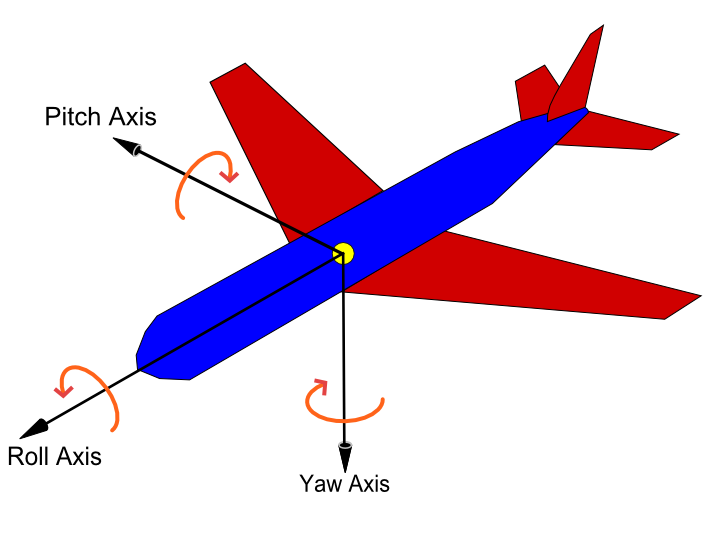
\includegraphics[width=0.45\linewidth]{Figures/Plane_Axes}
\caption{Aircraft body axes}
\label{fig:Plane_Axes}
\end{figure}


The derivative of the position is
\begin{IEEEeqnarray}{rCl} \label{eq:posDot}
	\dot{\bm{p}} &= & \bm{R}_b^T \bm{v_b}
\end{IEEEeqnarray}
We denote with $R_b$ the transformation matrix \textbf{from the Inertial frame to the Body frame}. Its elements are:

\begin{equation}
\bm{R}_b = \begin{bmatrix}
	\cos \theta \cos \psi                             & \cos\theta \sin\psi                               & -\sin\theta         \\
	-\cos\phi \sin\psi + \sin\phi \sin\theta \cos\psi & \cos\phi \cos\psi + \sin\phi \sin\theta\sin\psi   & \sin\phi \cos\theta \\
	\sin\phi \sin\psi + \cos\phi \sin\theta \cos\psi  & -\sin\phi \cos\psi + \cos\phi \sin\theta \sin\psi & \cos\phi \cos\theta
\end{bmatrix}
\end{equation}


Equation \eqref{eq:posDot} can be broken down onto its three elements as
\begin{IEEEeqnarray}{rCl}
	\dot{n} &= &(\cos \theta \cos \psi) u + (-\cos\phi \sin\psi + \sin\phi \sin\theta \cos\psi) v \nonumber\\
	&& +\> (\sin\phi \sin\psi + \cos\phi \sin\theta \cos\psi)w \IEEEyessubnumber \\
	\dot{e} &= & (\cos\theta \sin\psi)u + (\cos\phi \cos\psi + \sin\phi \sin\theta\sin\psi)v  \nonumber\\
	&& +\> (-\sin\phi \cos\psi + \cos\phi \sin\theta \sin\psi)w \IEEEyessubnumber \\
	\dot{d} &= & (-\sin\theta)u + (\sin\phi \cos\theta)v + (\cos\phi \cos\theta)w \IEEEyessubnumber
\end{IEEEeqnarray}

We see that the rotation matrix $\bm{R_B}$ is dependent upon three variables, $\phi$ , $\theta$ and $\psi$ . These are explained below.

\section{Orientation}

We use Euler angle notation to express the orientation of the aircraft. Roll, pitch and yaw are denoted as $\phi$, $\theta$ and $\psi$ respectively.
\begin{equation}
	\bm{\Phi} = [\phi \ \theta \ \psi]^T
\end{equation}

Figure \ref{fig:Euler_Anlges_2} has a visual representation of those angles. Take a note at the order of rotations: the standard order for aircraft applications, in order to come up with the body frame $\mathcal{F}_B$, starting from the NED frame is:
\begin{enumerate}
\item Rotate around NED z-axis by angle $\psi$, producing frame $\mathcal{F}_1$
\item Rotate around $\mathcal{F}_1$ y-axis by angle $\theta$, producing frame  $\mathcal{F}_2$
\item Rotate around  $\mathcal{F}_2$ x-axis by angle $\phi$, producing the $\mathcal{F}_B$ frame
\end{enumerate}
This convention is called the \emph{Tait-Bryan angles} \cite{Berner2008}

\begin{figure}[H]
\centering
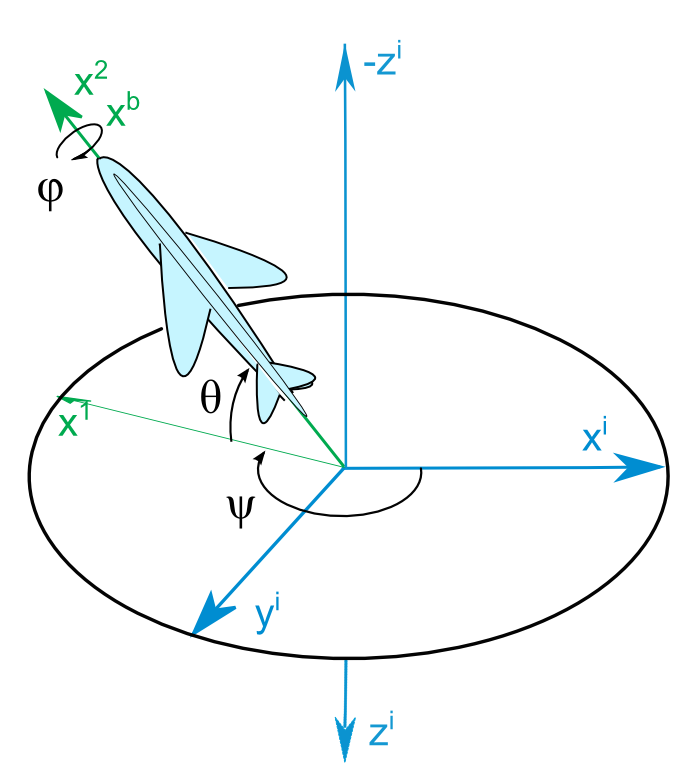
\includegraphics[width=0.35\linewidth]{Figures/Euler_Anlges_2}
\caption{Euler angles}
\label{fig:Euler_Anlges_2}
\end{figure}


The time derivative of the Euler angles is
\begin{equation}
	\dot{\bm{\Phi}} = \mathcal{E}(\bm{\Phi})\bm{\omega_b}
\end{equation}
where $\mathcal{E}(\bm{\Phi})$ is a rotation matrix, dependent upon the current orientation.

The individual angle propagation equations are
\begin{IEEEeqnarray}{rCl}
	\dot{\phi} & = & p + \tan\theta \sin\phi q + \tan\theta \cos\phi r \IEEEyessubnumber \\
	\dot{\theta} &= & \cos\phi q - \sin\phi r \IEEEyessubnumber \\
	\dot{\psi} &= & \frac{\sin\phi}{\cos\theta} q + \frac{\cos\phi}{\cos\theta} r \IEEEyessubnumber 
\end{IEEEeqnarray}

and equivalenty, $ \mathcal{E}(\bm{\Phi})$ is written as
\begin{equation}
\mathcal{E}(\bm{\Phi}) = \begin{bmatrix}
	1 & \tan \theta \sin \phi        & \tan \theta \cos \phi       \\
	0 & \cos \phi                    & -\sin \phi                  \\
	0 & \frac{\sin\phi}{\cos\theta} & \frac{\cos\phi}{\cos\theta}
\end{bmatrix}
\end{equation}

\section{Angular velocity}

We define the angular velocity vector as
\begin{equation}
	\bm{\omega} = [p\ q\ r]^T
\end{equation}

and its time derivative is
\begin{equation}  \label{eq:angVelDer}
	\dot{\bm{\omega}} = \frac{1}{\bm{J}}\left(\bm{T_b} - \bm{\omega} \times (\bm{J} \bm{\omega_b})\right)
\end{equation}
This equation incorporates the inertia matrix $\bm{J}$ and the input torque, expressed in the body axes $T_b$.

By spreading out the lines of the above vector equation we get

\begin{IEEEeqnarray}{rCl}
	\dot{p} &= & \frac{1}{\Gamma} \left[J_{xz} (J_x - J_y + J_z)pq - (J_z(J_z-J_y)+J_{xz}^2)qr + J_z T_x + J_{xz}T_z\right] \IEEEyessubnumber \\
	\dot{q} &= & \frac{1}{J_y} \left[(J_z - J_x)pr - J_{xz}(p^2 - r^2)+ T_y\right] \IEEEyessubnumber \\
	\dot{r} &= & \frac{1}{\Gamma} \left[((J_x - J_y)J_x + J_{xz}^2)pq - J_{xz}(J_x - J_y + J_z)qr + J_{xz}T_x + J_x T_z\right] \IEEEyessubnumber
\end{IEEEeqnarray}

To facilitate the calculation of cross products we may use this identity:
\begin{equation}
	\bm{\omega}\times \bm{v} = \begin{bmatrix}
		0  & -r & p  \\
		r  & 0  & -p \\
		-q & p  & 0
	\end{bmatrix} \bm{v}
\end{equation}
Where $\bm{v}$ is an arbitrary vector. Similarly,
\begin{equation}
	\bm{\omega} \times (\bm{\omega} \times \bm{v}) = \begin{bmatrix}
		-r^2-q^2 & pq & pr \\
		pq & -p^2 -r^2 & qr\\
		pr & qr & -p^2-q^2
	\end{bmatrix} \bm{v}
\end{equation}

The inertia matrix is defined as
\begin{equation}
	\bm{J} =
	\begin{bmatrix}
		\int(y^2 + z^2)~dm & -\int xy~dm        & -\int xz~dm        \\
		-\int xy~dm        & \int(x^2 + z^2)~dm & -\int yz~dm        \\
		-\int xz~dm        & -\int yz~dm        & \int(x^2 + y^2)~dm
	\end{bmatrix}
\end{equation}
Commonly, the inertia matrix in fixed-wing aircraft is considered to have zero elements in the x-y and y-z direction, since they are symmetric about the x-z plane.
\begin{equation}\label{eq:inertiaMat}
	\bm{J} = 
	\begin{bmatrix}
		J_x     & 0   & -J_{xz} \\
		0       & J_y & 0       \\
		-J_{xz} & 0   & J_z
	\end{bmatrix}
\end{equation}
	
\begin{equation}
	\Gamma = J_x J_z - J_{xz}^2
\end{equation}


\section{Linear Velocity}

We define linear velocity and its components as
\begin{equation}
	\bm{v_b} = [u\ v\ w]^T
\end{equation}

Its time derivative is
\begin{equation}
	\dot{\bm{v_b}} = -\bm{\omega_b} \times \bm{v_b} + \frac{\bm{F_b}}{m}
\end{equation}

which is equivalent to
\begin{IEEEeqnarray}{rCl}
	\dot{u} &= & rv -qw + \frac{F_bx}{m} \IEEEyessubnumber \\
	\dot{v} &= & -ru + pw + \frac{F_by}{m} \IEEEyessubnumber \\
	\dot{w} &= & qu -pv + \frac{F_bz}{m} \IEEEyessubnumber
\end{IEEEeqnarray}

We need to define the wind velocity, in the body frame. This is the velocity of the air-mass, moving above the ground, expressed in the body axes.
\begin{equation}
	\bm{v_w} = [u_w\ v_w\ w_w]^T
\end{equation}

The resulting relative (air)speed of the aircraft is
\begin{equation}
	\bm{v_r} = \bm{v}_B - \bm{v}_w
\end{equation}

Relative velocity is a very important quantity in aeronautics, as every aspect of the aircraft's aerodynamic response depends on it, rather than the inertial speed.

Based on the relative velocity, we define three more quantities:
\begin{itemize}
\item the angle of attack, $\alpha$
\item the angle of sideslip, $\beta$
\item the airspeed, $V_a$
\end{itemize}


\begin{IEEEeqnarray}{rCl}
	\alpha &= &\tan^{-1} \left(\frac{w_r}{u_r}\right) \IEEEyesnumber \IEEEyessubnumber \\
	\beta &= &\sin^{-1}\left(\frac{v_r}{V_a}\right) \IEEEyessubnumber \\
	V_a &= &\lVert[u_r\ v_r\ w_r]^T\rVert
\end{IEEEeqnarray}

Using these angles, a new frame of reference can be constructed, the Stability frame $\mathcal{F}_S$. The relative speed components (expressed in the body frame) can be constructed from the airspeed (expressed in the stability frame) using the following rotation:

\begin{equation}
\bm{v}_r = \bm{S}^T \begin{bmatrix}
V_a \\ 0 \\ 0
\end{bmatrix}
\end{equation}

\begin{equation}\label{eq:StabMatrix}
	\bm{S}=
	\begin{bmatrix}
		\cos\alpha \cos\beta & \sin\beta & \sin\alpha \cos\beta \\
		-\cos\alpha \sin\beta & \cos\beta & -\sin\alpha \sin\beta \\
		-\sin\alpha & 0 & \cos\alpha
	\end{bmatrix}
\end{equation}



\section{Mass Distribution}

It is useful to model the mass distribution of our aircraft. It has a nominal mass $m_{nom}$, placed at the center of gravity, the origin of the body axes. Any extra weights, such as payloads, debris, or component detachment can be modeled with extra masses $m_i$. Under this definition, $m_i$ is allowed to be negative.

\begin{IEEEeqnarray}{rCl}\label{eq:masses}
	m &= & m_{nom} + \sum m_i \IEEEyesnumber \IEEEyessubnumber \\
	\bm{p}_{m,nom} &= &[0\ 0\ 0]^T \IEEEyessubnumber \\
	\bm{p}_{CG} &= & \frac{1}{m} \left( \sum \bm{p}_i m_i\right)
\end{IEEEeqnarray}

Naturally, mass additions also affect the matrix of inertia of the aircraft. A mass $m_{e}$ planed at the point $p_{e} = [x_{e}, y_{e}, z_{e}]^T$ perturbs the matrix of inertia by
\begin{equation}
	\Delta \bm{J} =
	\begin{bmatrix}
		y_{e} z_{e} m_{e}  & -x_{e} y_{e} m_{e} & -x_{e}z_{e}m_{e}   \\
		-x_{e} y_{e} m_{e} & x_{e} z_{e} m_{e}  & -y_{e} z_{e} m_{e} \\
		-x_{e}z_{e}m_{e}   & -y_{e} z_{e} m_{e} & x_{e} y_{e} m_{e}
	\end{bmatrix}
\end{equation}
However, this perturbation in the matrix of inertia has not been incorporated into the angular velocity derivatives equations (\ref{eq:angVelDer}), for reasons of simplicity. 

\section{Wind Disturbances}
Another interesting model, primarily for simulation of autopilot software, is the one describing wind disturbances. It incorporates two sub-models: one for describing the constant wind velocity, as a function of altitude and one for producing wind turbulence. Static wind is intuitively expressed in the inertial frame, while turbulence is usually expressed in the body frame, so care is required in order to avoid confusion and errors in notation and coding.

\begin{equation}
	\bm{v_w} = \bm{v_{ws}} + \bm{v_{wg}}
\end{equation}

We denote with $\bm{v_{ws}}$ the constant wind vector, with components.

\begin{equation}
\bm{v_{ws}} = \bm{R}_B^T[v_{ws,n}, v_{ws,e}, v_{ws,d}]^T
\end{equation}

Usually we consider the vertical component of the wind to be zero ($v_{ws,d}=0$)

Another useful expression for constant wind is:
\begin{equation}
\bm{v_{ws}} = \bm{R}_B^TV_{ws}[-\cos\theta_w, -\sin\theta_w, 0]^T
\end{equation}
where $V_{ws}$ is the wind overall magnitude (in $m/s$) and $\theta_w$ is the wind direction (0degrees for North wind)

This allows us to introduce an altitude model for the wind magnitude, commonly known as the Power Law:
\begin{equation}
V_{ws} = V_{ws,h_r} \left(\frac{h}{h_r}\right)^\alpha
\end{equation}
This formula describes the increase of the wind magnitude as an exponential function of the altitude, given a measurement of wind magnitude $V_{ws,h_0}$ at altitude $h_0$. $\alpha$ is the Hellmann exponent (roughness exponent), which describes the wind shear effect. Commonly, surface wind magnitude measurements are available for the altitude of 10m, so the above formula becomes.
\begin{equation} \label{eq:staticWind10}
V_{ws} = V_{ws,h_{10}} \left(\frac{h}{h_{10}}\right)^\alpha
\end{equation}

Values for $\alpha$ vary with terrain morphology and wind turbulence. Some indicative values can be found in references \cite{Banuelos-Ruedas2011}, \cite{Peterson1978}, \cite{wiki:WindGrad}, \cite{wiki:Wind_profile_power_law}, but it is also claimed that the "1/7th power law" (using a value $\alpha=1/7$) is an adequate approximation for most purposes.
It should be noted, however, that most of the reviewed studies where oriented towards wind farm applications and wind models where validated up to a few hundred meters above ground.

The following table is pulled from \cite{Banuelos-Ruedas2011}

\begin{table}[H]
\centering
\begin{tabular}{|c|c|}
	\hline
	           Landscape type             & Friction coefficient $\alpha$ \\ \hline
	 Lakes, ocean and smooth hard ground  &              0.1              \\ \hline
	      Grasslands (ground level)       &             0.15              \\ \hline
	    Tall crops, hedges and shrubs     &             0.20              \\ \hline
	        Heavily forested land         &             0.25              \\ \hline
	Small town with some trees and shrubs &              0.3              \\ \hline
	 City areas with high rise buildings  &              0.4              \\ \hline
\end{tabular} 
\caption{Hellmann Exponent Values over Various Terrain}
\end{table}

An alternative model for wind shear can be found in \cite{Moorhouse1982}

Wind gusts can be modeled using Dryden transfer functions, as presented in \cite{Moorhouse1982}, \cite{BEAL1993}, \cite{MathWorks:DrydenTurbulence} and \cite{Beard2012} . Time responses can be generated by feeding unit variance white noise in the following filters. Note that airspeed is a parameter for these functions, but it can be replaced with the mean or cruise airspeed of the aircraft.
\begin{equation}
	\bm{V_{wg}}(s) =
	\begin{bmatrix}
		\sigma_u \sqrt{\frac{2V_a}{\pi L_u}} \frac{1}{s + \frac{V_a}{L_u}}\\
		\sigma_v \sqrt{\frac{3V_a}{\pi L_v}} \frac{s+\frac{V_a}{\sqrt{3}L_v}}{(s+\frac{V_a}{Lu})^2} \\
		\sigma_w \sqrt{\frac{3V_a}{\pi L_w}} \frac{s+\frac{V_a}{\sqrt{3}L_w}}{(s+\frac{V_a}{L_w})^2}
	\end{bmatrix}
\end{equation}

% Read BEAL1993 and verify the results

Typical values for the transfer function parameters for a small UAV can be found in \cite{Langelaan2011} and are copied below.
\begin{table}[H]
\centering
\begin{tabular}{|p{5cm}|c|c|c|c|c|}
	\hline
	            Description              & altitude (m) & $L_u$ (m) & $L_w$  (m) & $\sigma _u$ (m/s) & $\sigma _w$ (m/s) \\ \hline
	   low altitude, light turbulence    &      50      &    200    &     50     &       1.06       &       0.7        \\ \hline
	 low altitude, moderate turbulence   &      50      &    200    &     50     &       2.12       &       1.4        \\ \hline
	 medium altitude, light turbulence   &     600      &    533    &    533     &       1.5        &       1.5        \\ \hline
	medium altitude, moderate turbulence &     600      &    533    &    533     &       3.0        &       3.0        \\ \hline
\end{tabular} 
\caption{Gust Field Properties}
\end{table} %Kinematic Equations
\chapter{Dynamic Equations}

In this chapter the forces and moments exerted on the aircraft will be presented. The main dynamic components are gravity, aerodynamic reactions and propulsion (also referred to as thrust).
\begin{equation}
	\bm{F}_b = \bm{F}_g + \bm{F}_a + \bm{F}_t
\end{equation}

Before proceeding to any definitions, it is worth mentioning the control input variables. In normal airplane configurations, there are four control dimensions which the pilot can affect. These correspond to three sets of control surfaces (aileron, elevator and rudder) and the throttle command. The notation for these control variables is $\delta_a, \delta_a, \delta_t, \delta_r$. Essentially, these are the input variables to the aircraft model.$\delta_a, \delta_e,$ and $\delta_r$ are usually expressed in degrees of deflection from the neutral (zero) angle and $\delta_t$ is normalized in the (0,1) range.
Conventions for the positive direction of each control surface are not always consistent. In this text, the proposed positive direction of a control surface is the one which results in a positive moment around each primary axis (aileron - roll right, elevator - pitch up, rudder - yaw right).

\section{Gravity}

In this take, we assume a constant value for the acceleration of gravity, $g=9.805416m/s^2$ \cite[p.~8]{USStdAtm76}. The magnitude of the acceleration of gravity normally varies with altitude and geodetic coordinates, but a constant value is a valid approach for low altitude flight; unmodeled components are negligible to an adequate accuracy. The orientation of the gravity vector is always vertical, towards the center of the Earth, thus in the z-direction in the NED frame.
\begin{equation}
	\bm{F}_{g} = \bm{R}_b
	\begin{bmatrix}
		0\\ 0 \\mg
	\end{bmatrix}
\end{equation}
\begin{IEEEeqnarray}{rCl}
	\bm{F}_{gx} &= &-\sin \theta ~m g \IEEEyessubnumber\\
	\bm{F}_{gy} &= & \sin \phi \cos \theta ~m g  \IEEEyessubnumber\\
	\bm{F}_{gz} &= & \cos \phi \cos \theta ~m g \IEEEyessubnumber
\end{IEEEeqnarray}

\begin{equation}\label{eq:gravity}
	g = g_0
\end{equation}


\section{Aerodynamics}
This is the defining part of the flight characteristics of an airplane. The aerodynamic response of the airplane is crucial for its stability as well as its maneuverability.
Aerodynamic forces are presented in two frames of reference. The first is the body frame, whose corresponding forces, $\bm{F_a}$ are used for kinematic calculations. 
\begin{equation}
	\bm{F_a} = \begin{bmatrix}
	F_{ax} \\ F_{ay} \\ F_{az}
	\end{bmatrix}
\end{equation}
Aerodynamic forces are considered to be exerted, under normal operation, at the \emph{center of lift} ($\bm{p}_{CoL}$), a point located on the symmetry plane of the aircraft at one-quarter of the main wing chord.

However, for both historical and practical reasons, the flight characteristics of the airplane and the resulting forces (lift, drag and sideforce) are expressed in the stability frame (see eq.\ref{eq:StabMatrix}). Models of aircraft aerodynamics are also parametrized so as to predict the aerodynamic forces in the stability frame as well.

\begin{equation}
	\bm{F_s} = \begin{bmatrix}
	-F_D \\ F_Y \\ -F_L
	\end{bmatrix}
\end{equation}

Thus, we can obtain $\bm{F}_a$ via the equation
\begin{equation}
	\bm{F}_a = \bm{S}^T \bm{F}_s
\end{equation}
\begin{IEEEeqnarray}{rCl}
	F_{ax} &= & -\cos \alpha F_D -\cos \alpha \sin \beta F_Y + \sin \alpha F_L \IEEEyessubnumber\\
	F_{ay} &= & -\sin \beta F_D + \cos \beta F_Y \IEEEyessubnumber \\
	F_{az} &= & -\sin \alpha \cos \beta F_D -\sin \alpha \sin \beta F_Y - \cos \alpha F_L \IEEEyessubnumber
\end{IEEEeqnarray}

Aerodynamic moments need not be modeled in the stability frame. However, forces are generally not applied on the center of gravity of the aircraft, thus we need to model the moment they apply on it separately.
Sources of such additional moments are the stability margin (how much forward than the center of lift lies the center of mass), height difference between center of mass and center of lift (for example in a high-wing aircraft) and mass additions and subtractions to the airframe.

\begin{equation}
	\bm{T_a} = \begin{bmatrix}
		T_{ax} \\ T_{ay} \\ T_{az}
		\end{bmatrix}
		+\left(\bm{p}_{CoL} - \bm{p}_{CG}\right) \times \bm{F}_a
\end{equation}
\begin{IEEEeqnarray}{rCl}
	T_{ax,tot} &= & T_{ax} -dz F_{ay} + dy F_{az}\IEEEyessubnumber\\
	T_{ay,tot} &= & T_{ay} +dz F_{ax} - dx F_{az}\IEEEyessubnumber\\
	T_{az,tot} &= & T_{az} -dy F_{ax} + dx F_{ay}\IEEEyessubnumber
\end{IEEEeqnarray}

The next step in exploring the aerodynamic model is the definition of dynamic pressure. This quantity expresses the pressure exerted by the air moving around the airplane per unit of surface. It is proportional with the density of the air and with the square of the airspeed. Dynamic pressure is a crucial scaling factor for the rest of the aerodynamic equations
\begin{equation}
	\bar{q} = \frac{1}{2}\rho V_a^2
\end{equation}

The air density, $\rho$, is dependent upon altitude but its sea level value is adequate for numeric calculations ($\rho_0 = 1.225 kg/m^3$)

At this point we are able to express the force components as the product of dynamic pressure, the wing surface $S$, and the aerodynamic coefficients of lift, drag and sideforce, $C_L$, $C_D$, $C_Y$. It is very important to appreciate that these coefficients are not constant values; instead, they are functions of the state of the flying body, albeit their dependence from some state variables is more dominant than others. A more detailed explanation is given further down.
\begin{IEEEeqnarray}{rCl}
	F_D &= &\bar{q} S C_D \IEEEyesnumber \IEEEyessubnumber \\
	F_Y &= &\bar{q} S C_Y \IEEEyessubnumber\\
	F_L &= &\bar{q} S C_L \IEEEyessubnumber
\end{IEEEeqnarray}
\begin{IEEEeqnarray}{rCl}
	C_D &= &C_D(\alpha, q, \delta_e) \IEEEyesnumber \IEEEyessubnumber \\
	C_Y &= &C_Y(\beta, p, r, \delta_a, \delta_r) \IEEEyessubnumber\\
	C_L &= &C_L(\alpha, q, \delta_e) \IEEEyessubnumber
\end{IEEEeqnarray}

The aerodynamic moments are defined in a similar fashion, with the additional inclusion of wingspan $b$ and wing chord $c$. The notation for the moment coefficients may vary from source to source.
\begin{IEEEeqnarray}{rCl}
	T_{ax} &= &\bar{q} S b C_l \IEEEyesnumber \IEEEyessubnumber \\
	T_{ay} &= &\bar{q} S c C_m \IEEEyessubnumber\\
	T_{az} &= &\bar{q} S b C_n \IEEEyessubnumber
\end{IEEEeqnarray}
\begin{IEEEeqnarray}{rCl}
	C_l &= &C_l(\beta, p, r, \delta_a, \delta_r) \IEEEyesnumber \IEEEyessubnumber \\
	C_m &= &C_m(\alpha, q, \delta_e) \IEEEyessubnumber\\
	C_n &= &C_n(\beta, p, r, \delta_a, \delta_r) \IEEEyessubnumber
\end{IEEEeqnarray}

Finally, a model for the aerodynamic coefficients is provided. Undoubtedly, the most common and established approach is to use multivariable polynomials which are linear with respect to their coefficients. This representation lends itself nicely for parameter identification techniques, such as least-squares flavours, very common in real-world aircraft design and testing.
\begin{IEEEeqnarray}{rCl} \label{eq:forceCoeff}
	C_D &= & C_{D0} + C_{D\alpha} \alpha + C_{Dq} \frac{c}{2V_a}q + C_{D\delta_e} \delta_e \IEEEyesnumber \IEEEyessubnumber \\
	C_Y &= & C_{Y0} + C_{Y\beta} \beta + C_{Yp} \frac{b}{2V_a}p + C_{Yr}\frac{b}{2V_a}r + C_{D\delta_a} \delta_a + C_{Y\delta r} \delta_r \IEEEyessubnumber \\
	C_L &= & C_{L0} + C_{L\alpha} \alpha + C_{Lq}\frac{c}{2V_a}q + C_{L\delta_e} \delta_e \IEEEyessubnumber 
\end{IEEEeqnarray}

\begin{IEEEeqnarray}{rCl} \label{eq:torqueCoeff}
	C_l &= & C_{l0} + C_{l\beta} \beta + C_{lp}\frac{b}{2V_a}p + C_{lr}\frac{b}{2V_a}r + C_{l\delta_a} \delta_a + C_{l\delta_r} \delta_r \IEEEyesnumber \IEEEyessubnumber \\
	C_m &= & C_{m0} + C_{m\alpha} \alpha + C_{mq} \frac{c}{2V_a}q + C_{m\delta_e} \delta_e \IEEEyessubnumber \\
	C_n &= & C_{n0} + C_{n\beta} \beta + C_{np} \frac{b}{2V_a}p + C_{nr}\frac{b}{2V_a}r + C_{n\delta_a} \delta_a + C_{n \delta_r} \delta_r \IEEEyessubnumber
\end{IEEEeqnarray}

The coefficients which correspond to state variables ($C_{D\alpha}$,$C_{Dq}$,$C_{Y\beta}$,$ C_{Yp}$, $C_{Yr}$,$C_{L\alpha}$,$C_{Lq}$,$C_{l\beta}$,
$C_{lp}$,$C_{lr}$,$C_{m\alpha}$,$C_{mq}$,$C_{n\beta}$,$C_{np}$,$C_{nr}$) in most cases have values such that the resulting forces and moments tend to revert the aircraft to straight and level flight. Hence they are called \emph{stability derivatives}.

On the other hand, coefficients which correspond to the input variables ($C_{D\delta e}$,$C_{D\delta a}$,$ C_{Y\delta r}$,
$C_{L\delta e}$,$C_{l\delta_a}$,$C_{l\delta_r}$,$C_{m\delta_e}$,$C_{n\delta_a}$,$C_{n \delta_r}$) describe how the aircraft responds to control inputs and are hence called \emph{control derivatives}

Not all of the above derivatives need to be used in the formulation of the aerodynamic model of a plane. Some of them might be statistically insignificant for certain airframes (\cite{Klein2006}). On the other hand, longitudinal quantities usually do not incorporate coefficients of coefficients of lateral quantities and vice versa. This is in-line with the effort of decoupling the aircraft dynamics into a longitudinal and lateral plane, as much as possible, but there also are physical reasons, stemming from the aircraft geometry.


\section{Propulsion}

In the case of fixed-wing aircraft, most of the times the thrust is provided by a single propeller, acting upon the longitudinal axis of the aircraft, placed either in the front or the back of the fuselage. This discussion mainly draws from \cite[p.~127]{Allerton2009} but extends its contents from other sources to adapt to an electric power plant.
Propeller placement does not have an impact on the set of equation which form the model, even in the case of twin-propeller configurations, mounted on the wings.

Usually, thrust is considered to be produced only along the body x-axis, however, this approach may lack realism: it is not uncommon for the propeller to be mounted slightly tilted right and downwards, in order to minimize the counter-moment it produces and which affects the aircraft negatively.

\begin{equation} \label{eq:thrustForce}
	\bm{F}_t = \begin{bmatrix}
		F_{tx} \\ F_{ty} \\ F_{tz}
	\end{bmatrix}
\end{equation}

In case the propeller axis is aligned with the x-axis of the body frame, the following is also true:
\begin{IEEEeqnarray}{rCl} 
	F_{ty} &= & 0 \IEEEyessubnumber \\
	F_{tz} &= & 0 \IEEEyessubnumber
\end{IEEEeqnarray}

Naturally, the motor and propeller produce moments. Similarly to the aerodynamic moment analysis, we also have to take into account the displacement of the trust vector from the x-axis of the body frame.
\begin{equation} \label{eq:thrustTorque}
	\bm{T_t} = \begin{bmatrix}
		T_{tx} \\ T_{ty} \\ T_{tz}
	\end{bmatrix}
	 + (\bm{p}_{prop}-\bm{p}_{CG})\times \bm{F}_p
\end{equation}
\begin{IEEEeqnarray}{rCl}
	T_{tx,tot} &= & T_{tx} -dz F_{ty} + dy F_{tz}\IEEEyessubnumber\\
	T_{ty,tot} &= & T_{ty} +dz F_{tx} - dx F_{tz}\IEEEyessubnumber\\
	T_{tz,tot} &= & T_{tz} -dy F_{tx} + dx F_{ty}\IEEEyessubnumber
\end{IEEEeqnarray}


We opt to consider in our model only the aforementioned counter-moment produced in the x-axis by the propeller and motor, and not gyroscopic effects caused by the spinning propeller disc:
\begin{IEEEeqnarray}{rCl} 
	T_{ty} &= & 0 \IEEEyessubnumber \\
	T_{tz} &= & 0 \IEEEyessubnumber
\end{IEEEeqnarray}

With the aforementioned assumptions, the moment equations can be simplified into
\begin{IEEEeqnarray}{rCl}
	T_{ax,tot} &= & T_{tx}\IEEEyessubnumber\\
	T_{ay,tot} &= & dz F_{ax}\IEEEyessubnumber\\
	T_{az,tot} &= & -dy F_{ax}\IEEEyessubnumber
\end{IEEEeqnarray}

In order to build a detailed and useful thrust model for our aircraft, it is common to break it down into two main components: The propeller, along with its aerodynamic characteristics (after all, it is an airfoil operating inside the atmosphere), and the power plant. In this document, due to the author's research interests, a model for an electric power plant will be presented, comprised of an electric brushless motor, an Electronic Speed Controller (ESC) and a battery.

\subsection{Propeller Model}

Much like the aerodynamics of the airplane lifting surfaces, propeller thrust is dependent upon a coefficient function ($C_T$), the air density ($d$) and its scale (propeller diameter $D$). Additionally, it is proportional to the square of its rotational speed ($n$, in revolutions per second).

\begin{IEEEeqnarray}{rCl}
	F_{tx} &= & C_T \rho n^2 D^4 \\
	n &= & \frac{\omega_p}{2 \pi}
\end{IEEEeqnarray}

This time, the coefficient of thrust function has only one variable, the \emph{advance ratio} ($J$). This quantity is the ratio of the aircraft airspeed to the speed the propeller "screws" itself into the air volume. It is a means to quantify how efficiently the propeller forces itself into the air volume. $C_T$ generally doesn't have a simple shape. It is usually given by propeller manufacturers as a data set, which peaks at the nominal advance ratio and falls off at either side of the advance ratio range. This function can adequately model propeller stall, as well as the windmilling effect.

\begin{IEEEeqnarray}{rCl}
	C_T &=  & C_T(J) \label{eq:propCT}\\
	J &= & \frac{V_a}{nD}
\end{IEEEeqnarray}

In a similar fashion, there is an expression for the power that is consumed by the propeller in order to produce thrust and it uses a coefficient of power ($C_P$).

\begin{IEEEeqnarray}{rCl}
	P_p &= & C_P \rho n^3 D^5\\
	C_P & = & C_P(J)\label{eq:propCP}
\end{IEEEeqnarray}

A detail included in this model, not mentioned in most resources, is the equation which describes how the rotational speed of the propeller changes transiently in time. This is a differential equation of the rotational speed as a function of the difference between the available power from the motor ($P_e$) and the power consumed by the propeller. A necessary parameter is the moment of inertia along the x-axis of the whole engine-rotor and propeller system, which is summed up in the term $J_p$.

\begin{IEEEeqnarray}{rCl}
	\dot{n} &= & \frac{1}{J_p} \frac{P_e - P_p}{n}
\end{IEEEeqnarray}

Finally, the expression of propeller moment is simply derived from the ratio of the propeller power over the propeller rotational speed.

\begin{IEEEeqnarray}{rCl}
	T_{tx} &= & \frac{P_p}{\omega_p}
\end{IEEEeqnarray}

\subsection{Electric Motor Model}

The most wide-spread motor used in small UAVs is brushless outrunner permanent magnet electrical motor. Usually a 3-constant model is used, but for the sake of completeness, a 4-constant model will be used here, as presented in \cite{Carri2007}.

The input to the motor is the driving voltage, $V_{in}$ and the output is the output power, $P_e$. Naturally, if there is a direct-drive configuration between the motor and the propeller, the motor rotational speed ($n$, in revolutions per second) is the same as that of the propeller.

\begin{IEEEeqnarray}{rCl}
	n &= & K_v E_i \label{eq:motorKV}\\
	E_i &= & V_{in} - I_m R_m \label{eq:motorRM}\\
	P_e &= & E_i I_i \\
	I_i &= & I_m - I_0 - \frac{E_i}{R_1} \label{eq:motorR1}\\
	P_{in} &= & V_{in}I_m
\end{IEEEeqnarray}

\subsection{Battery and Electronic Speed Controller}

Finally, an expression for the overall combination of the battery and ESC is given.
\begin{itemize}
\item $V_{bat}$ is the internal battery voltage
\item $R_{bat}$ is the battery internal resistance
\item $R_S$ is the ESC in-line resistance
\item $\delta_t$ is the throttle command, essentially modulating the output voltage
\end{itemize}

\begin{IEEEeqnarray}{rCl}
	V_{in} &= & (V_{bat} - I_o (R_{bat} + R_S)) \delta_t \label{eq:battR}
\end{IEEEeqnarray} %Dynamic Equations
\chapter{Sensory Equipment Equations} \label{chap:Sensors}

In this chapter, the equations that describe the measurements of the various quantities and states via hardware sensors are laid out. Sensors often times use complicated physical phenomena to obtain a measurement of the desired quantity and sometimes the conversion process isn't straightforward. An effort to document relevant information is done here. No effort to model measurement errors is done here.
Most of the following device descriptions correspond to their MEMS versions.

\section{Inertial Measurements}
The first and perhaps most used family of sensors in robotics are the inertial sensors. Fusing them allows the extraction of instantaneous orientation and acceleration data which in turn enables dead-reckoning. This is a sensor suite with large cumulative error, but with very high bandwidth, suitable for attitude control. In this chapter, we assume that the sensor axes are aligned with the body axes perfectly. A good source of relevant information is \cite[p.25]{Stevens2003}.

\subsection{Accelerometer}
An accelerometer installed onboard the aircraft measures the body-frame accelerations \textbf{except} the acceleration of gravity. As a result, when the aircraft is laid to rest on the ground the sensor records acceleration with magnitude of 1G, even though the aircraft isn't moving at all. This is similar to the apparent feeling a human has, feeling the force of his weight pulling him down when resting but feeling weightless while in free-fall.

In the ideal case where the accelerometer is installed at the center of gravity of the aircraft, the recorded acceleration is

\begin{IEEEeqnarray}{rCl} \label{eq:bootstrap}
	\bm{a}_{b,m} &= &\bm{a}_b - \bm{R}_b\bm{g}\\
	 &=  & \frac{\bm{F}_b}{m} - \bm{R}_b \bm{g} \IEEEyessubnumber
\end{IEEEeqnarray}

However, this is an ideal case. Most of the times, the sensor is placed in a point with coordinates $\bm{r}_{acc}$ relative to the center of gravity. The resulting measurement, affected by the aircraft rotational velocity will be

\begin{equation}
	\bm{a}_{b,m} =  \frac{\bm{F_b}}{m} -  \bm{R}_b\bm{g} + \dot{\bm{\omega}}_b \times \bm{r}_{acc} + \bm{\omega}_b \times (\bm{\omega}_b \times \bm{r}_{acc}) \IEEEyessubnumber \\
\end{equation}
which can be expanded into
\begin{IEEEeqnarray}{rCl}
	a_{m,x} &= & \frac{F_x}{m}+g\sin\theta -\dot{r}r_{acc,y}+\dot{q}r_{acc,z}+(-r^2-q^2)r_{acc,x}+pqr_{acc,y}+prr_{acc,z} \IEEEyessubnumber\\
	a_{m,y} &= & \frac{F_y}{m}-\sin\phi\cos\theta +\dot{r}r_{acc,x}-\dot{p}r_{acc,z}+pqr_{acc,x} + (-p^2-r^2)r_{acc,y} +qrr_{acc,z}\IEEEyessubnumber\\
	a_{m,z} &= & \frac{F_z}{m}-\cos\phi\cos\theta -\dot{q}r_{acc,x}+\dot{p}r_{acc,y}+prr_{acc,x}  +qrr_{acc,y} + (-p^2-q^2)r_{acc,z}\IEEEyessubnumber
\end{IEEEeqnarray}
The angular velocity derivatives can be further substituted using eq~\ref{eq:angVelDer}.
\subsection{Gyroscope}
Gyroscopes are sensors capable of measuring the rotational velocities of the rigid body they are attached onto. This measurement is unaffected by the location of placement.
\begin{equation}
	\bm{\omega_m} = \bm{\omega_b}
\end{equation}

\subsection{Magnetometer}
Magnetometers are sensors which measure the magnetic field of the Earth. At any given point on the surface of the Earth the vector field components are known and thus this sensor can be used to extract orientation information. The intensity of the magnetic field (measured usually in nanoTesla) is mostly constant, at about 45~000~nT. However, the direction of the magnetic flux lines changes radically from location to location \cite{wiki:declination}, \cite{wiki:inclination}, \cite{NOAAGeom}. If we express the magnetic field intensity as a vector quantity with North, East and Down components, for a given pair of coordinates
\begin{equation}
\bm{h} = [h_N, h_E, h_D]^T
\end{equation}

then we define as declination the angle
\begin{equation}
	dec = \tan^{-1}\left(\frac{h_E}{h_N}\right)
\end{equation}
and the inclination as
\begin{equation}
	inc = \tan^{-1}\left(\frac{h_D}{\sqrt{h_N^2 + h_E^2}}\right)
\end{equation}

The measurement of the onboard magnetometer will then be
\begin{equation} \label{eq:magField}
	\bm{h}_m = \bm{h}_b =\bm{R}_b \bm{R}_{inc}\bm{R}_{dec} \begin{bmatrix}
			\lvert \bm{h} \rvert \\ 0 \\ 0
	\end{bmatrix}
\end{equation}

\subsection{AHRS}
There also are hardware solutions which incorporate all three aforementioned sensors and extract an estimation of the Euler angles set.
\begin{equation}
	\bm{\Phi_{m}} = \bm{\Phi}
\end{equation}

\section{GPS Measurements}
In order to have a reading of the absolute position of the aircraft in the inertial frame, be it the local NED frame or the global frame, defined by latitude and longitude, a GPS sensor is required. This is the only reasonable option, as radio-location is not a viable option for low-cost and low-weight robotic platforms. Whether the system will use a simple GPS receiver, a multi-constellation receiver, differential measurements or even RTK packages improves only the measurement accuracy.

Common quantities reported by a GPS receiver are the longitude, latitude and altitude set. However, these do not correspond to the NED frame. In order to translate them to the north, east and down quantities we need to obtain the data on the curvature of the Earth at the location of interest. The following discussion should be adequate for the needs of a NED frame spanning a few kilometers to each direction of the starting coordinates.

\subsection{Earth Model}
This discussion draws from \cite{Mulaire2000}, specifically chapter 3 and equations of p.~7.5.
According to the WGS-84, the Earth is modeled as an ellipsoid which is flatter on the poles and symmetric on the z-axis (the Earth's rotation axis). The semi-major axis is
\begin{equation}\label{eq:majorAxis}
	a=6~378~137m
\end{equation}
and the flattening, defined as
\begin{equation}
	f = \frac{a-b}{a}
\end{equation}
is equal to
\begin{equation}
	\frac{1}{f} = 298.257222101
\end{equation}
$b$ is the semi-minor axis of the ellipsoid and is calculated from the above equations and is equal to
\begin{equation}
	b=6~356~752.3142m
\end{equation}
The first eccentricity, $e$, is defined as
\begin{equation}
	e^2=2f-f^2
\end{equation}

With these constants available, for any given point on the surface of the Earth with latitude $\phi$, we can calculate the radius of curvature in the prime vertical
\begin{equation}
	R_N=\frac{a}{\sqrt{1-e^2\sin^2\phi}}
\end{equation}
and the curvature in the meridian
\begin{equation}
	R_M = \frac{a(1-e^2)}{(1-e^2\sin^2\phi)^{3/2}}
\end{equation}

Finally, a small change of latitude $\Delta \phi$ causes a shift in the north-south direction
\begin{equation}
	\Delta n = R_M \sin \Delta \phi
\end{equation}
and a small change of longitude $\Delta \lambda$ causes a shift in the east-west direction
\begin{equation}
	\Delta e = R_N \sin \Delta \lambda
\end{equation}

For such small angles (in the order of hundredths of a degree), the simplification $\sin \Delta \phi = \Delta \phi$ (in radians) might be acceptable.

For reference, at a latitude of 45degrees, a change of 0.01degree to the North corresponds to a distance of 1111.318m and the same change Eastwards corresponds to 1115.062m.

\textbf{Sidenote:} As of writing, the Google Earth 7.1.2 application for Linux reports a distance of about 1113m between the coordinates (45.00,00.00) and (45.01,00.00) and (curiously) a distance of about 788m(!) between the coordinates (45.00,00.00) and (45.00,00.01). Until further investigation, this results seems to be erroneous.

In case simpler calculations are required, one could use the geometric mean of the semi-major and semi-minor axis
\begin{equation}
	\bar{R} = \sqrt{a*b}
\end{equation}
and multiply it by the change in angle, regardless of direction.
\begin{equation}
	\Delta n = \bar{R} \Delta \phi
\end{equation}
For the previous example, the above equation yields 1111.327m, which is very acceptable for many applications.

Regarding altitude, GPS receivers report their vertical distance from the surface of the ellipsoid. Since the local NED frame is placed at the starting altitude, this altitude ($h_0$) should be used to initialize the frames. One could take altitude into account when calculating Cartesian displacements in the NED frame. This is as simple as adding altitude to the local Earth radius. This is demonstrated below.

Summing up, we do the following steps to convert from geodetic coordinates to local coordinates:
\begin{enumerate}
	\item Note the starting coordinates $\phi_0$, $\lambda_0$ and altitude $h_0$
	\item Calculate the radii of curvature $R_N(\phi_0)$ and $R_M(\phi_0)$
\end{enumerate}
For each GPS reading $(\phi, \lambda, h)$
\begin{enumerate}
	\item Calculate the differences $\Delta \phi = \phi - \phi_0$, $\Delta \lambda = \lambda - \lambda_0$ and $\Delta h = h - h_0$
	\item Calculate $n = (R_M + h) \sin \Delta \phi$
	\item Calculate $e = (R_N + h) \sin \Delta \lambda$
	\item Calculate $d = -\Delta h$
\end{enumerate}

Having done the above necessary conversions, we can treat the GPS receiver as a sensor which reports displacement in the local NED frame
\begin{equation}
	\bm{p_{gps}} = \bm{p}
\end{equation}

Additionally, most GPS receivers report ground velocities
\begin{equation}
	v_{gps} = \lVert [\dot{n}\ \dot{e}]' \rVert
\end{equation}
and the direction of travel, also referred to as the \emph{course angle}
\begin{equation}
	\chi_{gps} = \operatorname{atan2}\left({\dot{e}},{\dot{n}}\right)
\end{equation}


\section{Atmospheric Measurements}

\subsection{Atmosphere Model}
The primary resource for atmospheric models is \cite{USStdAtm76}. This technical report is the most accessible and adequately complete document among its "competitors". It provides models for all of the components of the atmosphere, ranging from temperature gradients to molecular synthesis of the air. It partitions the atmosphere into several layers, but we are interested only in the first one, spanning from 0m to approximately 11km. This range in adequate for the majority of UAV operations.

\textbf{Note}: The following discussion uses the gravitational model from \cite[eq.~17]{USStdAtm76}. This model differs from the one presented in \cite{Mulaire2000} in a noticeable way. \cite{USStdAtm76} uses the \emph{Standard Gravity} for the gravitational acceleration on the surface of the Earth, established by the International Committee on Weights and Measures in 1901.
\begin{equation} \label{eq:stdGravity}
	g_0 = 9.80665~ m/s^2
\end{equation}
This number is used uniformly for all latitudes. It is known that this is a simplification. However, we can proceed to the rest of the calculations and if need arises, switch $g_0$ for the more detailed model from \cite[eq.~4-1]{Mulaire2000}.

Additionally, the US Standard Atmosphere gravity model with respect to altitude uses the inverse square law for gravity decay
\begin{equation} \label{eq:usstdatmGravAlt}
	g(Z) = g_0 \left(\frac{r_0}{r_0+Z}\right)
\end{equation}
where
\begin{itemize}
	\item $Z$ is the geometric altitude above the surface, as reported by GPS systems
	\item $r_0$ is the radius of the Earth at a latitude where $g_0$ takes its standard value of $9.80665~ m/s^2$
\end{itemize}
The respective altitude model in WGS-84 is given in equation (4-3), for relatively low altitudes. Again, one can opt to use that model.

Where all this matters, is in the definition of the \emph{geopotential altitude}, $H$. This is expressed in \emph{geopotential meters} ($m'$), a unit of altitude, lifting a mass by which, always requires the same amount of work, no matter at which altitude this work is performed. Essentially, this expresses how easier it gets to lift masses in the weakening gravity as altitude increases and, in turn, this affects how less densely atmosphere is packed as altitude increases.
\begin{equation} \label{eq:geopotentialAlt}
	H = \frac{1}{g_0}\int_{0}^{Z}g\cdot dZ
\end{equation}
Combining equations \ref{eq:stdGravity}, \ref{eq:usstdatmGravAlt} and \ref{eq:geopotentialAlt} we get the following conversion expressions between geometric and geopotential altitude
\begin{equation}
	H = \frac{r_0 \cdot Z}{r_0 + Z}
\end{equation}
\begin{equation}
	Z = \frac{r_0 \cdot H}{r_0 - H}
\end{equation}

Next, we need to include a temperature model as a function of altitude.
\begin{equation}
	T = T_0 + L_0 \cdot (H - H_0)
\end{equation}
where
\begin{itemize}
	\item $H_0$ is our initialization altitude
	\item $T_0$ is the temperature at our initialization altitude. Its nominal value at sea-level is $288.15~K$
	\item $L_0 = -0.0065~K/m$ is the temperature gradient
\end{itemize}
The equation above describes how temperature drops as altitude increases.

Finally, we can express the variation of barometric pressure as a function of geopotential altitude
\begin{equation}
	P = P_0\left( \frac{T_{0}}{T(H)} \right) ^ {\left( \frac{g_0 \cdot M_0}{R^* \cdot L_{0}} \right)}
\end{equation}
where
\begin{itemize}
	\item $P_0$ is the pressure at our initialization altitude. According to the US Standard Atmosphere, at sea-level its value is $P_0 = 101325~N/m^2 = 1013.25~mb$
	\item $M_0 = 0.0289644~kg/mol$ is the mean molecular weight of the air
	\item $R^* = 8.31432~N\cdot m / (mol \cdot K)$ is the gas constant
\end{itemize}

Most importantly, one can solve this equation for $H$ and obtain the geopotential altitude by measuring the barometric pressure.
\begin{equation}
	H = \frac{T_0}{L_0}	\left( \left(\frac{P}{P_0}\right)^{\frac{g_0\cdot M_0}{R^* \cdot L_0}} -1\right) + H_0
\end{equation}

Air density can be obtained from the air pressure model
\begin{equation}
	\rho = \frac{P \cdot M_0}{R^* \cdot T}
\end{equation}

\subsection{Pressure}
Having defined the atmospheric model, we can now introduce a barometer sensor, which measures the barometric pressure at the UAV altitude.
\begin{equation}
	P_{bar} = P
\end{equation}

\subsection{Temperature}
Also, thermometers are available, which record the atmospheric temperature and are necessary for the extraction of altitude, through pressure readings. Care is needed however, as electronics are known to warm-up and raise the temperature in the enclosed spaces they are placed. However, this discussion belongs to an fault analysis and will not be expanded upon here.
\begin{equation}
	T_m =  T 
\end{equation}
What will be noted here is the fact that thermometers can be used to measure the temperature of components as well, such as batteries, ESCs or motors and provide a health status of those components.

\section{Air Data}
For an efficient and safe aircraft flight, air data measurements are required. These measurements refer to airspeed $\lVert V_a \lVert$, angle of attack $\alpha$ and angle of sideslip $\beta$.

Airspeed is measured using Pitot tubes, which take into account Bernoulli's equation to convert dynamic air pressure into airspeed readings. Essentially, a barometer is used to perform this reading.
\begin{IEEEeqnarray}{rCl}
	P_{t} &= & P + \frac{\rho V_a^2}{2} \IEEEyesnumber \IEEEyessubnumber \\
	P_{t,m} &= & P_t  \IEEEyessubnumber \\	
\end{IEEEeqnarray}

Aerodynamic angles $\alpha$ and $\beta$ can be measured using appropriate instruments, such as wind vanes, but such sensors are seldom found in medium and small UAVs, due to their size and weight.

\begin{equation}
	\alpha_m = \alpha
\end{equation}
\begin{equation}
	\beta_m = \beta
\end{equation}

\section{Distance Measurement}
Instruments which measure the distance of the UAV from the ground belong to this category. Common types are ultrasonic sensors, laser range finders and LIDARs. Their range varies from a few meters to a few hundred meters and their price range varies accordingly. What all these sensors have in common is that their measurements have a fixed range, varying from $d_{rf,min}$, the minimum reading, up to $d_{rf,max}$, in terms of absolute magnitudes.
\begin{equation}
	d_{rf} = \left\{ \begin{array}{ll}
	d_{rf, min} &,d>d_{rf,min} \\
	d &,h \in [d_{rf,min}, d_{rf,max}] \\
	d_{rm,max} &,d<d_{rf,max}
	\end{array}
	\right.
\end{equation}
Some confusion may be caused by the direction of the comparison ranges, but keep in mind that using the NED frame, $d$ is negative when the airplane is above ground altitude.

\section{Voltage Measurement}
Voltage Measurement is a very useful means to assess the remaining energy capacity of an onboard battery. Even though the relation between remaining energy and output voltage is not linear, useful conclusions can be extracted.

In general, any voltage level can be measured by such an instrument
\begin{equation}
	V_{i,m} = V_i
\end{equation}

but in the specific case of the battery voltage measurement we have
\begin{equation}
	V_{B,m} = V_B - I_o R_B
\end{equation}

\section{Current Measurement}
Similarly to voltage measurements, current measurements are available as well. These are useful to monitor the power consumption of the aircraft and, in extension, are a valid means to approach the thrust produced by the power plant.

Usually, current sensors are placed on the battery leads, since their most common occurrence measures only DC current.
\begin{equation}
	I_{o,m} = I_o
\end{equation}

\section{Motor Angular Velocity Measurement}
Finally, a quantity with great informational content is the rotational velocity of the motor shaft. This can be measured with commercial RPM sensors and can provide information on the thrust produced or even the health status of the motor itself.
\begin{equation}
	n_{m} = n
\end{equation} %Sensors

%% APPENDICES %%%%%%%%%%%%%%%%%%%%%%%%%%%%%%%%%
\appendix


%% Bibliography Section %%%%%%%%%%%%%%%%%%%%%%%
\bibliographystyle{/home/georgezp/texmf/tex/bibtex/bst/plain.bst}
\bibliography{References}

\end{document}

